\documentclass[10pt,twocolumn]{article}
\usepackage[margin=0.75in,columnsep=0.25in]{geometry}
\usepackage{booktabs,graphicx,amsmath,hyperref,microtype,xcolor,caption,url}
\captionsetup{font=small,labelfont=bf,skip=3pt}
\hypersetup{colorlinks=true,linkcolor=blue!50!black,citecolor=blue!50!black,urlcolor=blue!50!black}
\setlength{\parskip}{2pt}
\title{\textbf{alpaca.swift: A Dependency-Free Swift/Metal\\Inference Runtime for Apple Silicon,\\and Scaling Its Prefill to Larger Models}}
\author{Torin Etheridge\\\small\texttt{github.com/torinriley/alpaca}}
\date{Technical report, November 2026}
\begin{document}
\twocolumn[
\maketitle
\begin{abstract}
\noindent
alpaca.swift is a from-scratch language-model inference runtime for Apple Silicon written in Swift with custom Metal kernels: no llama.cpp, MLX, Core ML or Python at run time. An earlier evaluation measured one model (SmolLM2-135M) on one machine and reported large speed-ups over llama.cpp. This report tests whether those results generalise, finds that they do not at 1.7B parameters, diagnoses why, and changes the prefill GEMM to fix it. On an Apple M5 (16~GB) we compare alpaca against llama.cpp on the same GGUF files for SmolLM2 135M, 360M and 1.7B in F16, Q8\_0 and Q4\_0. Before any change, alpaca prefills the 135M and 360M models 1.25--1.68$\times$ faster than llama.cpp at 512--2048 tokens, but at 1.7B it is 0.63--0.82$\times$ as fast. A profile shows the feed-forward GEMMs take 76\% of 1.7B prefill time and that the $64{\times}64$ tensor-operation tile was bound by DRAM traffic on large matrices. We then (i)~launch threadgroups so that concurrent ones share a weight tile, (ii)~use a $128{\times}64$ tile for large matrices on long chunks, and (iii)~add an optional cache of half-precision copies of quantised weights. Over three runs, each measured back-to-back against llama.cpp, 1.7B F16 prefill at 512--2048 tokens goes from 0.66--1.13$\times$ to 1.18--1.80$\times$ of llama.cpp, and 1.7B Q8\_0 with the cache reaches 1.11--1.37$\times$ (from 0.61--1.17$\times$). The 135M and 360M models are unchanged without the cache and 5--23\% faster with it. Decode speed, greedy outputs and the numerical error are unchanged. Prompts of 16 tokens remain slower than llama.cpp (0.31--0.91$\times$ at 1.7B). The two reduced-precision shortcuts used for speed change next-token distributions by a mean KL divergence of $\le 1.9\cdot10^{-6}$ nats, and Q8\_0 costs $\le 0.004$ nats and Q4\_0 0.09--0.15 nats relative to F16. Everything was measured on a single, not-idle machine, with large drift in absolute speed between runs; nothing was run on an iPhone and energy was not measured.
\end{abstract}
\vspace{6pt}
]

\section{Introduction}
On-device language-model inference on Apple hardware is dominated by a few runtimes: llama.cpp~\cite{llamacpp} (C/C++, with a Metal backend), MLX~\cite{mlx} (C++/Python array framework) and Core ML. For Swift developers each of these means a foreign-language dependency or a model-conversion step. alpaca.swift is an independent implementation intended to remove both: a Swift package that memory-maps a GGUF file, runs a Llama-style decoder with hand-written Metal kernels, and exposes an \texttt{async} streaming API.

The project's first evaluation used a single 135M-parameter model. A 135M model is a poor proxy for the models people want to run on a phone or laptop: its matrices are small, its decode step is dominated by launch overheads and attention, and a kernel tuned on it may not transfer. This report therefore asks three questions.
\begin{description}\setlength\itemsep{0pt}
\item[Q1] Do alpaca's speed results against llama.cpp hold at larger model sizes?
\item[Q2] What do alpaca's reduced-precision speed shortcuts cost in output quality, with proper statistics?
\item[Q3] What does 4- and 8-bit weight quantisation cost, and does throughput survive sustained load?
\end{description}
The answer to Q1 is negative for the code as it stood at the start of this study: Section~\ref{sec:why} says where the time goes, and Section~\ref{sec:scaling} changes the GEMM and re-measures. The answers to Q2 and Q3 are favourable.

\paragraph{Contributions.} (i)~A three-size, three-format speed comparison with llama.cpp on identical files, with the full results and a second independent pass (Section~\ref{sec:speed}). (ii)~A profile-based account of why the advantage disappears at 1.7B (Section~\ref{sec:why}). (iii)~A paired, position-matched precision ablation using KL divergence against the most precise configuration (Section~\ref{sec:ablation}). (iv)~The quantisation-quality and sustained-load measurements (Sections~\ref{sec:quality} and~\ref{sec:sustained}). (v)~Three changes to the prefill GEMM that make 1.7B prefill faster than llama.cpp at 128 tokens and above on this machine, with the measurements before and after (Section~\ref{sec:scaling}). All code, scripts, raw JSON and the model checksums are in the repository (Appendix~\ref{app:repro}).

\section{System overview}
\label{sec:system}
alpaca.swift implements the Llama decoder family: RMSNorm~\cite{rmsnorm}, rotary position embeddings~\cite{rope}, grouped-query attention~\cite{gqa}, a SwiGLU feed-forward block~\cite{swiglu}, and a byte-level BPE tokenizer~\cite{gpt2}, read from GGUF~\cite{gguf} files. Weights are used in place from the memory-mapped file: the whole mapping is wrapped as one no-copy \texttt{MTLBuffer}, so resident weight memory is about the file size. F16, Q8\_0 and Q4\_0 tensors are consumed directly by the kernels; activations stay unquantised.

\paragraph{Prefill.} Prompts are processed in chunks of up to 512 tokens. Projections use Metal~4 tensor operations (\texttt{matmul2d}) on Apple10-family GPUs (M5/A19) with half-precision operands and float32 accumulation (the \texttt{fast} mode); quantised matrices are first expanded, one matrix at a time, into a half-precision scratch buffer, or read from an optional half-precision cache built at load time (Section~\ref{sec:scaling}). Matrices with at least $2\cdot10^{6}$ weights processed in chunks of at least 256 tokens use a $128{\times}64$ output tile; everything else uses $64{\times}64$. Attention is a FlashAttention-style~\cite{flashattention} tiled kernel with online softmax and causal block skipping, with half-precision Q, K, V and P.

\paragraph{Decode.} One token is six fused dispatches per layer. Attention uses a split-K scheme in which one threadgroup handles all query heads that share a KV head, in the spirit of Flash-Decoding~\cite{flashdecoding}. Greedy decoding runs entirely on the GPU with several command buffers in flight.

\paragraph{Correctness baseline.} Every operation has a CPU reference. The repository's validation reports that the CPU backend matches Hugging Face float32 logits to $5\cdot10^{-5}$ (F16) and $7\cdot10^{-5}$ (Q8\_0), that 191/191 tokeniser test strings produce identical IDs, and that 72/72 greedy tokens match for each format on SmolLM2-135M; the GPU default configuration lies within $1.1\cdot10^{-3}$ of the logit peak. These figures are from the project documentation and were not re-derived here; Section~\ref{sec:ablation} adds the distribution-level view.

\section{Method}
\label{sec:method}
\paragraph{Hardware and software.} Apple M5 (10-core GPU), 16~GB unified memory, macOS 27.0.1, Swift 6.4, release build. llama.cpp is the Homebrew build 11429 (\texttt{d81235049}) with the Metal backend and \texttt{-ngl 99}; other settings are the defaults. The machine was an ordinary desktop session (load average 2--5 from a browser, the window server and background applications), not an isolated benchmark host.

\paragraph{Models.} SmolLM2-Instruct~\cite{smollm2} at 135M, 360M and 1.7B parameters, GGUF conversions by bartowski, in F16, Q8\_0 and Q4\_0 (SHA-256 sums in the repository). All three sizes share one tokeniser and architecture (Llama-style; the 1.7B model has full multi-head attention, 32 KV heads, while 135M and 360M use grouped-query attention with 3 and 5 KV heads). SmolLM2 was chosen because it is the only family in the supported set (no RoPE scaling, byte-level BPE with a supported pre-tokeniser, no biases) that spans more than one size. The 1.7B Q4\_0 file stores its embedding table as Q6\_K, which alpaca rejects by design; that cell is absent.

\paragraph{Speed protocol.} Both engines process the same files. Prefill throughput is prompt tokens divided by time to the first token's logits; decode throughput is $(g{-}1)$ generated tokens divided by the interval between first and last token, greedy, $g{=}64$. alpaca is timed through its public streaming API (\texttt{alpaca bench}); llama.cpp is timed with \texttt{llama-bench} (\texttt{-p}, \texttt{-n 64 -d}). Each cell is the median (alpaca) or mean (\texttt{llama-bench}) of 7 repetitions after a warm-up. Prompt lengths are 16, 128, 512, 2048; decode contexts are 16, 512, 2048. The \emph{whole} grid was run twice (pass~1 and pass~2) on different occasions. Because absolute speed drifted between passes (Section~\ref{sec:variance}), the figure of merit is the \textbf{ratio} alpaca/llama.cpp within a pass.

\paragraph{Quality protocol.} Per-position scoring on the WikiText-2~\cite{wikitext} raw test set (301{,}948 tokens). For each of $N$ positions $p$ spaced evenly through the text, the window of the preceding $L{=}256$ tokens is prefilled and the final-token logits score token $p$. This forces the \emph{prefill} kernels to produce the logits under test, but only one position per window is scored, so absolute perplexities are higher-variance and not comparable with published full-context numbers; we therefore report \emph{paired} differences on identical positions with percentile-bootstrap 95\% CIs (2000 resamples over positions). The precision ablation scores the same windows under four configurations of one model instance: \textsc{ref} (float32 KV cache, float32-operand \texttt{exact} GEMM), \textsc{gemm} (only half-precision GEMM operands), \textsc{kv16} (only the f16 KV cache) and \textsc{default}. We report $\Delta$NLL against \textsc{ref}, the mean KL divergence $\mathrm{KL}(p_{\textsc{ref}}\,\|\,p_{\textsc{cfg}})$ over the full vocabulary, and the fraction of positions whose arg-max token changes. One component, the half-precision Q/P inside the tiled attention kernel, cannot be switched off and is present in all four configurations, so \textsc{ref} is the most precise \emph{available}, not an all-float32 reference.

\paragraph{Baseline and scaling protocol.} Sections~\ref{sec:speed}--\ref{sec:variance} describe the code as it was at the start of the study (``base''). The GEMM changes of Section~\ref{sec:scaling} were measured by running, for each model and format, the base build, the new build, the new build with the prefill cache (quantised formats only) and \texttt{llama-bench}, one after another on the same file and prompt lengths, so that all four see the same machine state. The 1.7B models were measured in three separate runs (A, B, C) because the machine's state changed between them; the small models were measured once.

\paragraph{Profiles.} Per-stage GPU time from \texttt{alpaca profile}, which uses GPU timestamps at encoder boundaries; stages are serialised, so their sum can differ slightly from the unprofiled pass.

\section{Speed against llama.cpp (before the GEMM changes)}
\label{sec:speed}
\begin{table*}[t]\centering\small
\begin{tabular}{llrrrrrr}\toprule
 & & \multicolumn{3}{c}{prefill, tok/s (ratio)} & \multicolumn{3}{c}{decode, tok/s (ratio)}\\
\cmidrule(lr){3-5}\cmidrule(lr){6-8}
model & fmt & $n{=}16$ & 512 & 2048 & ctx 16 & 512 & 2048\\\midrule
135M & F16 & 2,437 (0.78) & 34,686 (1.64) & 26,054 (1.59) & 273 (1.13) & 252 (1.04) & 227 (1.04)\\
135M & Q8\_0 & 2,506 (0.57) & 30,073 (1.43) & 23,661 (1.47) & 467 (1.33) & 414 (1.24) & 358 (1.17)\\
135M & Q4\_0 & 3,112 (0.81) & 29,697 (1.32) & 23,802 (1.46) & 545 (1.37) & 481 (1.22) & 396 (1.16)\\

360M & F16 & 1,152 (0.95) & 12,527 (1.60) & 11,333 (1.68) & 112 (1.11) & 108 (1.11) & 95 (1.04)\\
360M & Q8\_0 & 958 (0.49) & 11,390 (1.25) & 9,938 (1.35) & 183 (0.95) & 198 (1.09) & 172 (1.04)\\
360M & Q4\_0 & 1,301 (0.61) & 11,791 (1.27) & 10,008 (1.36) & 293 (1.15) & 267 (1.06) & 213 (1.04)\\

1.7B & F16 & 307 (0.91) & 1,724 (0.79) & 1,623 (0.82) & 24 (0.98) & 23 (0.96) & 21 (0.88)\\
1.7B & Q8\_0 & 181 (0.33) & 1,676 (0.75) & 1,611 (0.79) & 47 (0.98) & 45 (0.95) & 40 (0.74)\\
1.7B & Q4\_0 & \multicolumn{6}{c}{not supported (Q6\_K embedding)}\\
\bottomrule\end{tabular}
\caption{Throughput of the base code (before the changes of Section~\ref{sec:scaling}; tokens/s, median of 7) and, in parentheses, its ratio to llama.cpp on the same file, pass~1. Prefill columns are prompt lengths, decode columns context lengths. Ratios above 1 favour alpaca. Pass~2 values are in Table~\ref{tab:repro} and the raw data.}
\label{tab:speed}
\end{table*}
\begin{figure*}[t]\centering
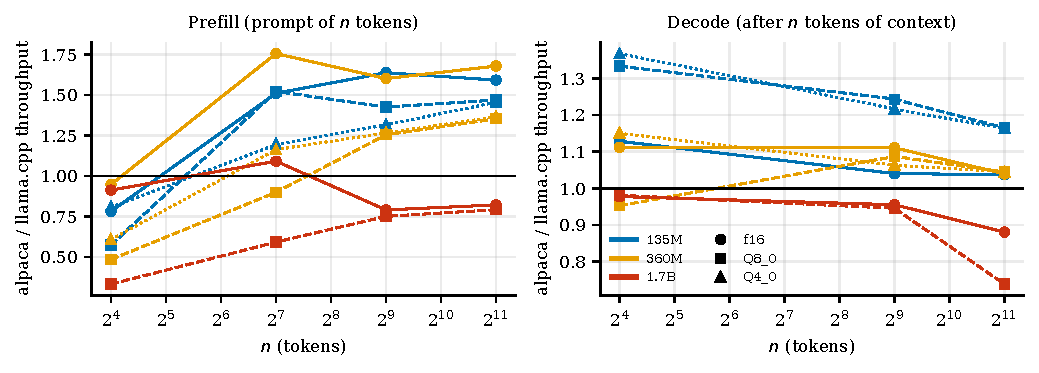
\includegraphics[width=0.82\textwidth]{figs/ratio.pdf}
\caption{alpaca/llama.cpp throughput ratio (pass~1) against prompt length (left) and context length (right). Colour is model size, line style and marker are weight format. Base code: the 1.7B model (red) falls below parity for prefill $\ge 512$ tokens; Table~\ref{tab:scaling} shows the result after the changes.}
\label{fig:ratio}
\end{figure*}
Table~\ref{tab:speed} and Figure~\ref{fig:ratio} give the results for the base code, i.e.\ before the changes of Section~\ref{sec:scaling}. Over both passes:
\begin{itemize}\setlength\itemsep{0pt}
\item \textbf{135M and 360M, prefill $\ge$512 tokens:} 1.25--1.68$\times$ llama.cpp in all 12 cells per pass. This reproduces the earlier 135M result (1.3--1.7$\times$).
\item \textbf{135M and 360M, short prompts ($n{=}16$):} 0.49--0.95$\times$; alpaca is slower, as the earlier report also found.
\item \textbf{135M and 360M, decode:} 0.95--1.39$\times$ across contexts 16--2048; the advantage shrinks with context (at 2048, 0.98--1.20$\times$).
\item \textbf{1.7B, prefill $\ge$512 tokens:} 0.63--0.82$\times$, i.e.\ alpaca is slower. At $n{=}16$ it is 0.31--0.91$\times$.
\item \textbf{1.7B, decode:} 0.74--1.01$\times$, roughly at parity except for one Q8\_0 cell at context 2048 (0.74$\times$ in pass~1, 1.01$\times$ in pass~2), which we regard as unresolved.
\end{itemize}

\section{Why the advantage did not scale (before the GEMM changes)}
\label{sec:why}
\begin{figure}[t]\centering
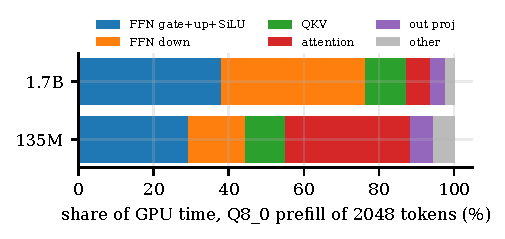
\includegraphics[width=\columnwidth]{figs/stages.pdf}
\caption{Share of GPU time per stage for a 2048-token Q8\_0 prefill. At 1.7B the two large feed-forward GEMMs dominate; at 135M attention is a third.}
\label{fig:stages}
\end{figure}
\begin{table}[t]\centering\small
\resizebox{\columnwidth}{!}{\begin{tabular}{llrrrr}\toprule
 & & \multicolumn{2}{c}{prefill TFLOP/s} & \multicolumn{2}{c}{decode GB/s}\\
\cmidrule(lr){3-4}\cmidrule(lr){5-6}
model & fmt & alpaca & llama.cpp & alpaca & llama.cpp\\\midrule
135M & F16 & 5.5 & 3.5 & 74 & 66\\
135M & Q8\_0 & 5.0 & 3.4 & 68 & 51\\
135M & Q4\_0 & 5.1 & 3.5 & 50 & 37\\
360M & F16 & 7.1 & 4.2 & 81 & 73\\
360M & Q8\_0 & 6.3 & 4.6 & 71 & 74\\
360M & Q4\_0 & 6.3 & 4.6 & 67 & 59\\
1.7B & F16 & 5.2 & 6.4 & 82 & 84\\
1.7B & Q8\_0 & 5.2 & 6.6 & 85 & 87\\
\bottomrule\end{tabular}}
\caption{Effective prefill matrix throughput at $n{=}2048$, computed as $2\times$ (matmul parameters) $\times$ tokens/s, and effective weight-streaming rate at decode context 16, computed as file bytes $\times$ tokens/s (pass~1). The FLOP count excludes attention and is therefore a lower bound.}
\label{tab:eff}
\end{table}
Figure~\ref{fig:stages} shows the Q8\_0 prefill profile at 2048 tokens. For 135M, attention is 33.3\% of GPU time, FFN gate+up 29.3\%, FFN down 15.1\% and QKV 10.6\%. For 1.7B, FFN down (38.2\%) and gate+up (38.1\%) together take 76\%, QKV 10.9\%, and attention only 6.4\%; the pass takes 1131~ms on the GPU. Prefill at 1.7B is therefore a pure large-GEMM problem.

Table~\ref{tab:eff} converts throughput to matrix FLOP/s. alpaca sustains 5.0--7.1 TFLOP/s on the projections at every size, with no increase at 1.7B (5.2 TFLOP/s). llama.cpp's rate grows with model size, from 3.4--3.5 (135M) through 4.2--4.6 (360M) to 6.4--6.6 TFLOP/s (1.7B), and overtakes alpaca at 1.7B. The F16 1.7B file is also slower (0.66--0.82$\times$ at $n\ge512$) even though F16 involves no weight expansion, so the quantised-weight scratch-expansion step is not the main cause. Our reading is that alpaca's tensor GEMM, which before this study had been developed and benchmarked only on the 135M model, does not keep improving as the matrices grow, while llama.cpp's does. This was a hypothesis when the profile was taken; Section~\ref{sec:scaling} tests it by changing the tile and the launch order.

Decode tells a simpler story. At context 16 both engines stream the weights at similar rates (82--87~GB/s at 1.7B, Table~\ref{tab:eff}), so decode is memory-bound and parity is expected; the GPU-side profile at 1.7B (15.5~ms per token, 117~GB/s of weight traffic) was taken in the faster machine state of pass~2. At context 2048 attention is 19\% of a 1.7B decode step (3.6 of 18.9~ms profiled) against 1.0\% at context 16, which is where any remaining attention-kernel gap would show; the model has 32 KV heads, so alpaca's sharing of K/V across a query-head group buys nothing there.

\section{Scaling the prefill GEMM}
\label{sec:scaling}
\paragraph{Diagnosis.} The base kernel computes a $64$-token $\times$ $64$-row output tile per threadgroup. Each tile reads about 2~MB of operands for 67~MFLOP, roughly 32~FLOP per byte, which is too little reuse for matrices whose weights do not fit in the GPU's caches. In addition, threadgroups were launched with the output-row tile varying fastest, so the threadgroups resident at one time read many different weight tiles and each weight tile was fetched again for every token tile. In the 1.7B Q8\_0 profile the FFN-down projection ran at about 4.5~TFLOP/s against about 10~TFLOP/s for gate+up. The 135M model's matrices are small enough to stay in cache, which hid all of this.

\paragraph{Changes.} (1)~\textbf{Launch order.} The token tile is now the fastest-varying grid axis, so concurrently running threadgroups use the same weight tile. (2)~\textbf{Larger tile.} A $128$-token $\times$ $64$-row tile (templated kernels, one source for both sizes) doubles the arithmetic intensity. It is chosen per matrix, only when the matrix has at least $2\cdot10^{6}$ weights and the chunk has at least 256 tokens, because an earlier version that used it everywhere slowed down the 135M and 360M models and short chunks. (3)~\textbf{Prefill weight cache.} With \texttt{--prefill-cache} (\texttt{LoadOptions.prefillWeightCache}), quantised projection matrices are expanded to half precision once at load, which removes the per-chunk expansion pass. It costs 2 bytes per weight of extra memory and is off by default; the loader refuses it if the estimate exceeds the memory budget.

\paragraph{Results.}
\begin{table*}[t]\centering\small
\begin{tabular}{llccccccccc}
\toprule
& & \multicolumn{3}{c}{Run A (earlier variant)} & \multicolumn{3}{c}{Run B} & \multicolumn{3}{c}{Run C (degraded)}\\
\cmidrule(lr){3-5}\cmidrule(lr){6-8}\cmidrule(lr){9-11}
Format & $n$ & base & new & cache & base & new & cache & base & new & cache\\
\midrule
F16  & 128  & 1.13 & 1.24 & --   & 1.16 & 1.16 & --   & 1.32 & 1.32 & --\\
F16  & 512  & 0.66 & 1.35 & --   & 0.77 & 1.57 & --   & 0.99 & 1.18 & --\\
F16  & 2048 & 0.70 & 1.36 & --   & 0.92 & 1.80 & --   & 1.13 & 1.23 & --\\
\addlinespace
Q8\_0 & 128  & 0.63 & 0.64 & 1.13 & 0.72 & 0.71 & 0.86 & 0.73 & 0.72 & 0.89\\
Q8\_0 & 512  & 0.61 & 1.01 & 1.35 & 0.98 & 1.09 & 1.18 & 0.93 & 1.04 & 1.11\\
Q8\_0 & 2048 & 0.67 & 1.06 & 1.33 & 1.17 & 1.26 & 1.37 & 1.06 & 1.15 & 1.29\\
\bottomrule
\end{tabular}

\caption{SmolLM2-1.7B prefill: alpaca/llama.cpp throughput ratio before (base) and after (new; cache = new with \texttt{--prefill-cache}), measured back-to-back with llama.cpp on the same file. Ratios above 1 favour alpaca. Run A used an earlier variant that applied the $128$-token tile to every matrix; runs B and C used the final adaptive rule. Run C was taken while the machine was degraded (llama.cpp's absolute speed was about half that of run B), which compresses the ratios.}
\label{tab:scaling}
\end{table*}
\begin{table}[t]\centering\small
\begin{tabular}{llccc}
\toprule
Model & Format & base & new & cache\\
\midrule
135M & F16  & 1.48 & 1.47 & --\\
135M & Q8\_0 & 1.33 & 1.34 & 1.48\\
135M & Q4\_0 & 1.33 & 1.34 & 1.45\\
360M & F16  & 1.48 & 1.50 & --\\
360M & Q8\_0 & 1.25 & 1.28 & 1.51\\
360M & Q4\_0 & 1.26 & 1.31 & 1.47\\
\bottomrule
\end{tabular}

\caption{135M and 360M prefill at $n{=}512$, alpaca/llama.cpp ratio before and after (single run).}
\label{tab:small}
\end{table}
Table~\ref{tab:scaling} gives the 1.7B results. At 512 and 2048 tokens F16 goes from 0.66--1.13$\times$ to 1.18--1.80$\times$ of llama.cpp; the run-to-run spread is large, but the new code is faster than llama.cpp in all three runs and faster than the base in every cell at these lengths. Q8\_0 without the cache reaches 1.01--1.26$\times$ (base 0.61--1.17$\times$), and with the cache 1.11--1.37$\times$. At 128 tokens, F16 is unchanged (the base was already ahead), and Q8\_0 improves only with the cache (0.86--1.13$\times$ against 0.63--0.73$\times$). The absolute throughput gain is the figure least affected by drift: in run B the F16 prefill at 512 tokens went from 1979 to 4048~tok/s on the same machine state.

Table~\ref{tab:small} shows that the smaller models are not hurt: without the cache the ratios are within 0.05 of the base, and the cache adds 5--23\% at 128 tokens and above (for example 360M Q8\_0 at 128 tokens, 1.16$\times$ to 1.43$\times$). Decode throughput is unchanged, as expected, since no decode kernel was touched.

\paragraph{Correctness.} Greedy decoding of 64 tokens after a prompt of roughly 400 tokens produced identical token sequences before and after, with and without the cache, for 360M Q8\_0, 1.7B Q8\_0 and 1.7B F16. The precision ablation of Section~\ref{sec:ablation} gives a mean KL of $1.4$--$1.9\cdot10^{-6}$ nats on the new build, the same as before. The repository's XCTest suite was not run on these changes.

\paragraph{What is still slower.} At 16 tokens alpaca remains behind llama.cpp: 0.31--0.91$\times$ at 1.7B (the worst case is Q8\_0, 0.31--0.38$\times$ with or without the cache) and 0.63--0.91$\times$ for the small models. The 16-token path does not use the large tile and reads quantised weights in two passes; a 16-token kernel that reads the quantised weights directly is the obvious next change and is not done. Also, without the cache 1.7B Q8\_0 is only near parity at 512 tokens and below parity at 128.

\section{Cost of the speed shortcuts}
\label{sec:ablation}
\begin{table*}[t]\centering\small
\begin{tabular}{llrrrr}\toprule
model/fmt & configuration & $\Delta$NLL [95\% CI] & mean KL & max KL & top-1 flips\\\midrule
1.7B F16 ($N{=}600$) & f16 GEMM operands & $-4.0$ [-15.2, +7.2]$\cdot10^{-5}$ & 0.58$\cdot10^{-6}$ & 28$\cdot10^{-6}$ & 0.00\%\\
1.7B F16 ($N{=}600$) & f16 KV cache & $-1.0$ [-14.1, +12.4]$\cdot10^{-5}$ & 0.94$\cdot10^{-6}$ & 35$\cdot10^{-6}$ & 0.00\%\\
1.7B F16 ($N{=}600$) & both (default) & $+5.9$ [-9.7, +21.1]$\cdot10^{-5}$ & 1.33$\cdot10^{-6}$ & 32$\cdot10^{-6}$ & 0.00\%\\
\midrule
135M Q4\_0 ($N{=}2000$) & f16 GEMM operands & $+3.8$ [-3.6, +12.1]$\cdot10^{-5}$ & 1.36$\cdot10^{-6}$ & 43$\cdot10^{-6}$ & 0.00\%\\
135M Q4\_0 ($N{=}2000$) & f16 KV cache & $-0.1$ [-5.5, +5.5]$\cdot10^{-5}$ & 0.61$\cdot10^{-6}$ & 42$\cdot10^{-6}$ & 0.10\%\\
135M Q4\_0 ($N{=}2000$) & both (default) & $+7.7$ [-2.2, +17.9]$\cdot10^{-5}$ & 1.88$\cdot10^{-6}$ & 24$\cdot10^{-6}$ & 0.05\%\\
\midrule
135M F16 ($N{=}2000$) & f16 GEMM operands & $-2.3$ [-9.8, +4.8]$\cdot10^{-5}$ & 0.86$\cdot10^{-6}$ & 38$\cdot10^{-6}$ & 0.05\%\\
135M F16 ($N{=}2000$) & f16 KV cache & $+1.0$ [-4.7, +7.3]$\cdot10^{-5}$ & 0.54$\cdot10^{-6}$ & 13$\cdot10^{-6}$ & 0.05\%\\
135M F16 ($N{=}2000$) & both (default) & $-3.3$ [-12.3, +5.1]$\cdot10^{-5}$ & 1.38$\cdot10^{-6}$ & 23$\cdot10^{-6}$ & 0.00\%\\
\midrule
360M F16 ($N{=}4000$) & f16 GEMM operands & $-3.7$ [-8.7, +1.0]$\cdot10^{-5}$ & 0.81$\cdot10^{-6}$ & 192$\cdot10^{-6}$ & 0.05\%\\
360M F16 ($N{=}4000$) & f16 KV cache & $+1.7$ [-2.7, +6.1]$\cdot10^{-5}$ & 0.71$\cdot10^{-6}$ & 81$\cdot10^{-6}$ & 0.05\%\\
360M F16 ($N{=}4000$) & both (default) & $-3.1$ [-9.1, +3.1]$\cdot10^{-5}$ & 1.41$\cdot10^{-6}$ & 155$\cdot10^{-6}$ & 0.00\%\\
\bottomrule\end{tabular}
\caption{Precision ablation against \textsc{ref} on identical positions ($N$ windows of 256 tokens). $\Delta$NLL is in units of $10^{-5}$ nats with bootstrap 95\% CIs; KL is the mean over positions of $\mathrm{KL}(p_{\textsc{ref}}\,\|\,p)$; flips is the share of positions whose arg-max changes.}
\label{tab:ablation}
\end{table*}
\begin{figure}[t]\centering
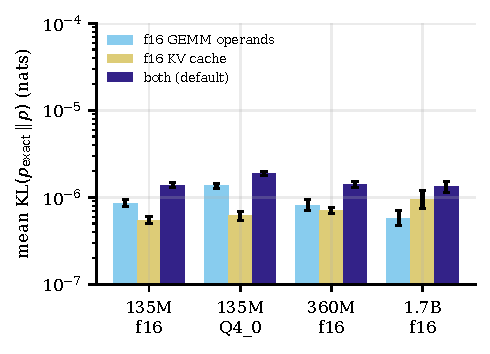
\includegraphics[width=0.93\columnwidth]{figs/kl.pdf}
\caption{Mean KL divergence (with bootstrap 95\% CIs) of each shortcut configuration from the most precise configuration.}
\label{fig:kl}
\end{figure}
Table~\ref{tab:ablation} and Figure~\ref{fig:kl} show that neither shortcut measurably changes the model. In all four model/format settings every $\Delta$NLL has a 95\% CI that includes zero, with point estimates below $10^{-4}$ nats. Mean KL is $5\cdot10^{-7}$ to $1.9\cdot10^{-6}$ nats and the worst single position has KL $\le 2\cdot10^{-4}$; the arg-max changes at 0--0.1\% of positions. The default (both shortcuts) has roughly the sum of the two individual KLs, as expected for independent rounding errors. The effect does not grow with model size over the range tested (135M to 1.7B) and is similar for Q4\_0 weights (mean KL $1.9\cdot10^{-6}$ against $1.4\cdot10^{-6}$ for F16 at 135M).

The cost of avoiding the shortcuts is large. Wall time to prefill one 256-token window under \textsc{ref} versus \textsc{default} was 41.3 vs 6.7~ms (135M, F16), 105.2 vs 18.0~ms (360M) and 312.9 vs 87.7~ms (1.7B): 3.6--6.2$\times$ slower. These timings were taken during the ablation runs under varying machine state and are indicative only. The conclusion is that the default configuration is a good trade at these sizes; the 1.7B ablation uses $N{=}600$ positions and so has wider intervals.

\section{Quantisation quality}
\label{sec:quality}
\begin{table}[t]\centering\small
\resizebox{\columnwidth}{!}{\begin{tabular}{llrlr}\toprule
model & fmt & PPL & $\Delta$NLL [95\% CI] & top-1\\\midrule
135M & F16 & 21.30 & -- & --\\
135M & Q8\_0 & 21.38 & +0.0041 [+0.0020, +0.0062] & 97.6\%\\
135M & Q4\_0 & 24.64 & +0.1457 [+0.1238, +0.1697] & 79.4\%\\
360M & F16 & 15.32 & -- & --\\
360M & Q8\_0 & 15.33 & +0.0006 [-0.0013, +0.0024] & 98.2\%\\
360M & Q4\_0 & 16.69 & +0.0855 [+0.0679, +0.1050] & 84.2\%\\
1.7B & F16 & 10.96 & -- & --\\
1.7B & Q8\_0 & 10.98 & +0.0012 [-0.0004, +0.0029] & 98.4\%\\
\bottomrule\end{tabular}}
\caption{Quantisation cost on WikiText-2 ($N{=}3000$ paired positions, default GPU configuration). PPL is the end-of-window perplexity (wide CIs; see text), $\Delta$NLL is paired against F16, and top-1 agree is the share of positions where the arg-max token matches F16.}
\label{tab:quality}
\end{table}
Table~\ref{tab:quality} reports paired costs. Q8\_0 is effectively free: $\Delta$NLL is $+0.0041$ nats for 135M (CI $[0.0020,0.0062]$) and statistically indistinguishable from zero for 360M and 1.7B, with 97.6--98.4\% top-1 agreement. Q4\_0 costs $+0.146$ nats at 135M and $+0.086$ at 360M (CIs exclude zero) with only 79.4\% and 84.2\% top-1 agreement; its cost shrinks with size, as is commonly observed. The 1.7B Q4\_0 file could not be evaluated. Absolute perplexities (21.3, 15.3, 11.0 for F16) have bootstrap CIs of about $\pm10\%$ because only one token is scored per window.

\section{Sustained load}
\label{sec:sustained}
\begin{figure}[t]\centering
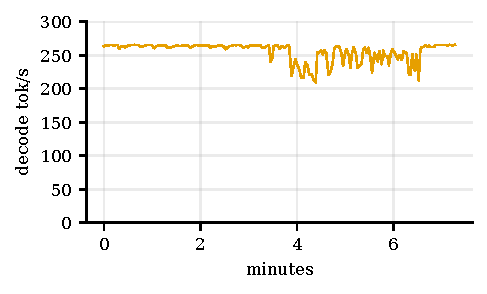
\includegraphics[width=0.93\columnwidth]{figs/sustained.pdf}
\caption{Decode throughput of SmolLM2-360M Q8\_0 over 199 back-to-back 512-token generations (about 7.3 minutes).}
\label{fig:sustained}
\end{figure}
Figure~\ref{fig:sustained} shows 199 consecutive 512-token generations on SmolLM2-360M Q8\_0 (about 7.3~minutes of continuous GPU work). Throughput does not decay: the mean of the first 20 runs is 264.1 tok/s and of the last 20 is 264.2 tok/s, and the reported thermal state stayed \emph{nominal}. Between roughly minutes 3.5 and 6.5, 55 of the 199 runs fell below 255 tok/s (minimum 209) before throughput recovered; we were running short analysis scripts on the same machine in that period and did not control for it, so we do not attribute the stretch to the GPU. A 200th run stalled for 302~s for a reason we did not identify (machine-level, not thermal) and is excluded; the run therefore covered about 7.3 rather than the planned 10 minutes. This is a Mac with active cooling. It says little about a phone, and neither power nor energy was measured.

\section{Variance and reproducibility (base code)}
\label{sec:variance}
\begin{table}[t]\centering\small
\begin{tabular}{llrrrr}\toprule
 & & \multicolumn{2}{c}{prefill ratio, $n{=}512$} & \multicolumn{2}{c}{decode ratio, ctx 512}\\
\cmidrule(lr){3-4}\cmidrule(lr){5-6}
model & fmt & pass 1 & pass 2 & pass 1 & pass 2\\\midrule
135M & F16 & 1.64 & 1.49 & 1.04 & 1.06\\
135M & Q8\_0 & 1.43 & 1.33 & 1.24 & 1.25\\
135M & Q4\_0 & 1.32 & 1.33 & 1.22 & 1.25\\
360M & F16 & 1.60 & 1.49 & 1.11 & 0.97\\
360M & Q8\_0 & 1.25 & 1.25 & 1.09 & 1.05\\
360M & Q4\_0 & 1.27 & 1.26 & 1.06 & 1.08\\
1.7B & F16 & 0.79 & 0.66 & 0.96 & 0.94\\
1.7B & Q8\_0 & 0.75 & 0.63 & 0.95 & 0.99\\
\bottomrule\end{tabular}
\caption{Ratio alpaca/llama.cpp at 512 tokens in two independent passes of the whole grid.}
\label{tab:repro}
\end{table}
Absolute throughput was not stable across passes: pass~2 was faster than pass~1 by a median factor of 1.33 (135M and 360M decode) to 1.36 (1.7B) for alpaca and 1.31--1.35 for llama.cpp. We did not identify the cause (clock or power state, or background load). Because the shift is common to both engines, ratios move much less (Table~\ref{tab:repro}): across the 8 model/format rows shown, the ratio changed by at most 0.15 in prefill and 0.14 in decode, never changing which engine was faster except at the 360M F16 decode (1.11 vs 0.97). Absolute tok/s should not be compared across passes or with the earlier report; the ratios are the transferable result. The 1.7B conclusion (below parity for prefill at $n\ge512$) holds in both passes.

\section{Limitations}
\begin{itemize}\setlength\itemsep{0pt}
\item \textbf{One machine, one OS build, not idle.} Nothing was run on an iPhone or iPad, so the paper's main motivating platform is untested; the fast prefill path needs M5/A19-class hardware.
\item \textbf{One model family.} Three sizes of SmolLM2 only. Llama~3.x models (RoPE scaling, different pre-tokeniser), K-quants and models with biases are rejected by alpaca; we cannot say how results look on them.
\item \textbf{Comparison protocol.} llama.cpp was a Homebrew build with default flags and was timed by its own benchmark tool; alpaca was timed through its public API. Tuned or newer llama.cpp builds, different flash-attention settings, or other engines (MLX) could change the ratios. alpaca does not quantise activations, llama.cpp does, so outputs are not bit-comparable.
\item \textbf{Quality protocol.} One scored token per window; short (256-token) context; one corpus. KL and $\Delta$NLL are paired and precise, absolute perplexity is not. The half-precision attention Q/P could not be ablated.
\item \textbf{Not measured:} energy, power, memory pressure under contention, models above 1.7B, batch sizes above one, long contexts (above 2048 tokens) in this study.
\item \textbf{Scaling study.} The 1.7B ratios vary by up to 0.6 between runs because machine state changed (run C was degraded), so the size of the gain is uncertain even though its sign is not. Run A used an earlier tile variant. The small models and the base/new comparison on them are a single run. The repository's XCTest suite was not run on the changes; correctness evidence is identical greedy output on three configurations and unchanged KL.
\item \textbf{Cache cost.} \texttt{--prefill-cache} adds 2 bytes per quantised weight, which may be unacceptable on phones; the 1.7B Q4\_0 file is unsupported and was not measured.
\end{itemize}

\section{Conclusion}
As originally written, alpaca.swift was a faster-than-llama.cpp prefill engine only for small (135M--360M) models on an M5; at 1.7B it was slower. A profile showed that the large feed-forward GEMMs were limited by memory traffic, and changing the launch order, using a larger tile for large matrices and optionally caching half-precision weights makes 1.7B prefill 1.2--1.8$\times$ (F16) and 1.1--1.4$\times$ (Q8\_0 with the cache) as fast as llama.cpp at 512 tokens and above on this machine, without changing decode, outputs or numerical error. Short prompts are still slower than llama.cpp, quantised formats need the cache to win at 128 tokens, and the gain was measured on one noisy machine. The next steps are a 16-token quantised kernel, a run on an idle machine and on an iPhone, energy measurement, and support for the model families people actually deploy.

\section*{Disclosure}
The experiments, analysis and first draft of this report were produced by an AI assistant (Claude) working under the author's instruction, from the repository's code and the measurements described here. The author is responsible for the content; all numbers are generated from the raw result files by the scripts in the repository.

\appendix
\section{Reproducing the results}
\label{app:repro}
\begin{small}
\begin{verbatim}
# models (bartowski GGUF) + wikitext-2 test text
# speed grid, both engines, same files:
Experiments/run_bench.sh <outdir> 135M 360M 1.7B
python3 Experiments/analyze_bench.py <outdir> \
        135M,360M,1.7B
# paired scoring / precision ablation:
.build/release/AlpacaEval <model.gguf> wiki.test.raw \
   --positions 3000 --window 256 \
   --configs ref,gemm,kv16,default --out out.json
python3 Experiments/analyze_eval.py
# profiles, drift pass, sustained decode:
Experiments/run_extra.sh
python3 Experiments/make_figs.py
python3 Experiments/make_tables.py
# scaling study (base/new/cache vs llama.cpp):
MODELS="135M 360M 1.7B" OUT=<dir> BASE=<base build> \
  Experiments/run_opt.sh
python3 Experiments/analyze_opt.py <dir>
\end{verbatim}
\end{small}
Raw JSON, logs, the environment record and model checksums are under \texttt{Experiments/results}.

\begin{thebibliography}{99}\small
\bibitem{llamacpp} G.~Gerganov et al. llama.cpp: LLM inference in C/C++. \url{https://github.com/ggml-org/llama.cpp}, 2023.
\bibitem{gguf} GGUF file format specification, ggml project. \url{https://github.com/ggml-org/ggml}.
\bibitem{mlx} A.~Hannun, A.~Hannun, et al. MLX: An array framework for Apple silicon. \url{https://github.com/ml-explore/mlx}, 2023.
\bibitem{smollm2} L.~Ben Allal et al. SmolLM2: When Smol Goes Big --- Data-Centric Training of a Small Language Model. arXiv:2502.02737, 2025.
\bibitem{flashattention} T.~Dao, D.~Fu, S.~Ermon, A.~Rudra, C.~R\'e. FlashAttention: Fast and memory-efficient exact attention with IO-awareness. NeurIPS 2022.
\bibitem{flashdecoding} T.~Dao, D.~Haziza, F.~Massa, G.~Sizov. Flash-Decoding for long-context inference. PyTorch blog, 2023.
\bibitem{gqa} J.~Ainslie et al. GQA: Training generalized multi-query transformer models from multi-head checkpoints. EMNLP 2023.
\bibitem{rope} J.~Su et al. RoFormer: Enhanced transformer with rotary position embedding. arXiv:2104.09864, 2021.
\bibitem{rmsnorm} B.~Zhang, R.~Sennrich. Root mean square layer normalization. NeurIPS 2019.
\bibitem{swiglu} N.~Shazeer. GLU variants improve transformer. arXiv:2002.05202, 2020.
\bibitem{gpt2} A.~Radford et al. Language models are unsupervised multitask learners. OpenAI technical report, 2019.
\bibitem{wikitext} S.~Merity, C.~Xiong, J.~Bradbury, R.~Socher. Pointer sentinel mixture models. arXiv:1609.07843, 2016.
\end{thebibliography}
\end{document}
